\subsection{Deuxième partie : Le drone}
\label{part:drone}
    \subsubsection{Drone : Généralités}
        \paragraph*{}
        Comme dit dans la partie \ref{part:existDrone}, le laboratoire possède 2 drones achetés récemment. Les deux drones sont identiques et ce sont les DJI Matrice 100\cite{matrice100}. Ces drones sont indiqués par le constructeur comme \textit{fait pour les développeurs}. Il y a ainsi de nombreuses applications possibles grâce à ces drones. La communication avec le drone se fait de diverses manières, selon ce que l'on veut faire. Par exemple, pour une utilisation classique d'un drone, il y a la télécommande de livrée et il est possible de diriger le drone grâce à cette télécommande; ou sinon, si on veut utiliser l'autopilote, il est possible de donner, grâce à l'application Android DJI Go, des points GPS au drone et il exécutera la course en suivant les points GPS donnés puis en retournant au point de départ. Ou enfin, une autre solution, celle que j'ai appliqué, c'est d'utiliser un ordinateur embarqué tel qu'un \rpi ~ou le Manifold\cite{manifold} qui est construit et développé par la même entreprise, DJI. L'avantage du \rpi ~sur n'importe quel autre ordinateur embarqué c'est la puissance disponible par rapport au prix. J'ai eu à disposition un \rpi ~3B+ (RPi3) qui comporte 1Go de RAM, processeur Cortex-A53 cadencé à 1.4GHz en 64 bits, avec tout un large éventail de connexions réseaux, une possibilité d'avoir une sortie vidéo et sonore. Aujourd'hui, un RPi3 coûte environ 68€ (avec carte SD, alimentation) ce qui est négligeable par rapport aux possibilités qu'il offre et surtout par rapport au rapport qualité/prix sur tous ses concurrents.
            
    \subsubsection{Drone : Équipements nécessaires}
        \paragraph*{}
        Afin d'effectuer les missions nécessaires au stage, il est utile d'utiliser un ordinateur embarqué tel que le \rpi ~cité précédemment. Une fois ce mini-ordinateur choisi, on peut imaginer le matériel nécessaire, par exemple le positionnement du drone dans la pièce. Nous avons un étage au dessus du plafond de la salle et énormément de matériel métallique dans la pièce utilisée, ce qui conduit à une impossibilité d'utiliser le GPS ainsi que la centrale inertielle (voir partie \ref{part:posiDrone}). De ce fait, nous avons utilisé des cartes Decawave fonctionnant en $UWB$ ce qui permet de positionner le drone rapidement en sachant que 12 cartes plus l'application afin d'utiliser ces cartes coutent 199\$.
        Enfin, nous avons besoin d'une caméra afin de prendre en photo les différents capteurs si l'on détecte une anomalie. Pour la caméra, le choix a été un peu long car il y a beaucoup de choix : GoPro, caméra DJI, caméra \rpi. Chacune de ces caméras avait leurs avantages et leurs inconvénients. La caméra DJI coûte très cher (entre 1000€ et 3000€) mais donne une image très nette car la caméra est stabilisée; la GoPro coûte bien moins cher mais reste onéreuse (330€ avec les fonctionnalités voulues); et la caméra du \rpi ~coûte bien moins cher encore mais n'est pas stabilisée donc des photos moins nette mais pour environ 57€. Au final, la GoPro était impossible à utiliser car la GoPro nécessitait une connexion WiFi pour communiquer avec le \rpi ~mais la communication WiFi était déjà prise sur la carte pour pouvoir accéder à la base de données sur l'ordinateur. Nous nous sommes donc orienté vers la caméra du \rpi ~car les fonctionnalités qu'elle possède nous suffisait et il est simple de capturer des images depuis un programme en C++.
        
    \subsubsection{Drone : Onboard-SDK (OSDK) sur \rpi ~et tests de communications}
        \paragraph{Connexion}
            \paragraph*{}
            L'outil de communication avec le drone fourni par DJI se nomme Onboard-SDK (OSDK). Il est utilisé dans un ordinateur embarqué (\rpi) connecté au drone.
            
            Tout d'abord, avant de pouvoir utiliser le OSDK sur le \rpi, il faut régler certains paramètres tels que le \textit{Baud Rate, la fréquence de transmission des capteurs et l'activation du contrôle par l'API}. Ceci se fait grâce à l'application DJI Assistant 2 fournie et s'installe sur un ordinateur (Windows, iOS). Le \textit{Baud Rate} est donc mis à 230400 et le reste sur 10Hz pour avoir une lecture des capteurs toutes les 100ms. Il serait possible de mettre plus rapide mais la consommation énergétique serait plus importante également.
            
            \paragraph*{}
            L'OSDK tourne sur Ubuntu (16.0) mais peut également tourner sur Raspbian (OS pour le \rpi ~dérivé de Debian). Le code du OSDK tourne sur le \rpi ~et récupère les valeurs du drone via l'$UART$. Le SDK permet d'accéder aux données des capteurs de manière automatisée, ainsi que de déplacer le drone (décollage et atterissage compris).
        
        \paragraph{Résultats}
            \paragraph*{}
            Une fois le OSDK installé et opérationnel sur le \rpi, j'ai pu exécuter les codes qui sont fournis en exemple. Sur la figure \ref{fig:exTelemetry}, l'exemple qui est montré ici est l'exemple où on interroge les capteurs de position (GPS), vitesse (centrale inertielle), \textit{RC Commands} correspond à la commande faite sur la télécommande (r : roll / p : pitch / y : yaw / thr : thrust).
        
            \begin{figure}[H]
                \centering
            	\begin{frame}{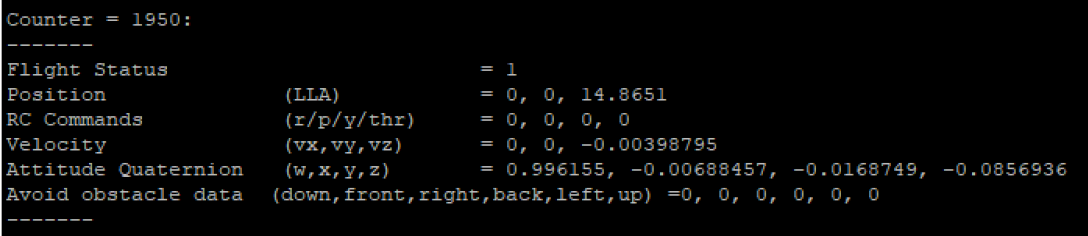
\includegraphics[width=1\textwidth]{image/telemetry.png}}
            	\end{frame}
            	\caption{\label{fig:exTelemetry}Exemple fournis par DJI}
            \end{figure}
        
    
    \subsubsection{Drone : Positionnement dans la pièce}
    \label{part:posiDrone}
        \paragraph*{}
        Afin de positionner le drone dans la pièce et étant donné que le GPS ne peut pas fonctionner dans la pièce, il est nécessaire d'utiliser un moyen externe. Nous avons ainsi choisi les cartes Decawaves MDEK1001 pour le positionnement. Tout d'abord, il faut créer le réseau avec les cartes. On crée donc un réseau grâce à l'application Android fournie (voir figure \ref{fig:network}) puis on y assigne nos cartes Decawaves en paramétrant la position par rapport à une carte initiale qui sera positionnée en {X = 0; Y = 0; Z = 0}. On obtient donc avec 7 cartes ancres et un tag ce que l'on peut voir sur la figure \ref{fig:listeCartes} et le placement des cartes dans l'environnement est représenté par la figure \ref{fig:placementVisuel}.
        
        \begin{figure}[H]
            \centering
        	\begin{frame}{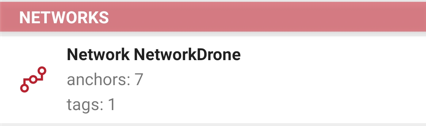
\includegraphics[scale=1]{image/UI_Decawave2.png}}
        	\end{frame}
        	\caption{\label{fig:network}Composition du réseau}
        \end{figure}
        
        \begin{minipage}[c]{0.45\linewidth}
            \begin{figure}[H]
                \centering
            	\begin{frame}{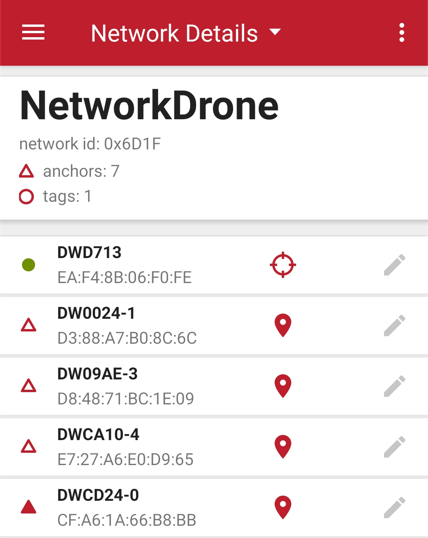
\includegraphics[width=1\textwidth]{image/UI_Decawave1.png}}
            	\end{frame}
            	\caption{\label{fig:listeCartes}Composition du réseau en détail}
            \end{figure}
        \end{minipage} \hfill
        \begin{minipage}[c]{0.45\linewidth}
            \begin{figure}[H]
                \centering
            	\begin{frame}{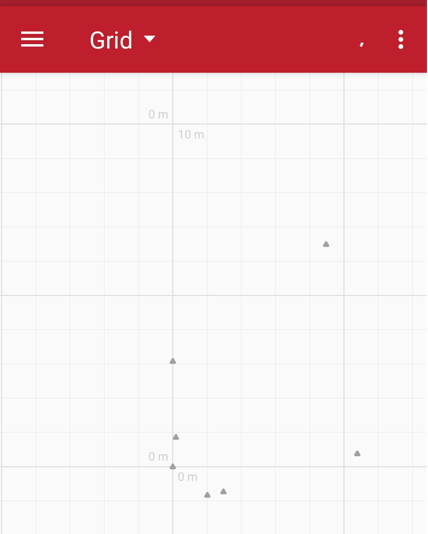
\includegraphics[width=1\textwidth]{image/UI_Decawave3.png}}
            	\end{frame}
            	\caption{\label{fig:placementVisuel}Placement visuel des cartes dans l'espace}
            \end{figure}
        \end{minipage}
        
        \paragraph*{}
        Une fois les cartes initialisées et le \rpi ~connecté à une carte Decawave, il est possible de récupérer les valeurs de position et de distance entre la carte du drone (tag) et les ancres positionnées.
        
        Il y a deux solutions possible. La première suffit d'aller sur l'application Android et de voir sur le grille la distance estimée du tag (Rappel : carte du drone). Mais cette solution n'est pas utile à long terme car ce que l'on désire c'est d'embarquer cette position et de diriger le drone en lui donnant cette position.
        
        Ainsi, j'ai utilisé la seconde solution qui est d'interroger le tag via la connexion USB. Une fois les 4 cartes connectées et initialisées, il est possible via la commande Linux : \textit{sudo minicom -D /dev/ttyACMO} d'accéder au moniteur série et d'exécuter des commandes spécifiques à l'appareil connecté. Dans mon cas, les commandes utiles sont :
        
        \begin{itemize}
            \item "\textit{lep}" montre la position sous forme : POS, positionX, positionY, positionZ, qualité du signal (en pourcentage)
            \item "\textit{les}" montre la distance entre le tag et les 4 ancres les plus proches. Exemple : 1151[5.00,8.00,2.25] = 6.48 0CA8[0.00,8.00,2.25] = 6.51 111C[5.00,0.00,2.25] = 3.18 1150[0.00,0.00,2.25] = 3.16 le\_us = 2576 est[2.57,1.98,1.68,100]
        \end{itemize}
        
        \paragraph*{}
        Une fois les valeurs de distances avec les cartes, nous avons pu établir des marges d'erreur et se rendre compte que la position estimée par Decawave (Méthode de Newton/Raphson) était avec une erreur de 10cms environ. J'ai donc voulu tester une méthode différente de celle implémentée dans la carte afin de vérifier s'il était possible d'avoir un meilleur résultat. La méthode de Decawave mettait une limitation dans le nombre de cartes qu'elle utilisait. En effet, il ne pouvait en aucun cas y avoir plus que 4 cartes Decawaves utilisées pour le calcul de la position. Or, normalement, plus le nombre de cartes est élevé et plus la précision est grande. C'est pourquoi, j'ai voulu voir avec la méthode de Bancroft qui prend un grand nombre de cartes; tout en faisant le comparatif entre les deux méthodes pour voir si j'obtenais de meilleurs résultats avec la contrainte de temps que j'avais : avoir une réponse toute les 100ms maximum !
        
        \paragraph*{}
        En exécution normale, le drone se déplace grâce aux données que calcule et lit le \rpi. Le programme qui tourne sur le \rpi ~est construit en multi thread. Un thread gère la communication avec le drone via le $SDK$ et l'autre thread gère le positionnement et le déplacement via les cartes Decawave.
        
        \paragraph{Méthode de Bancroft}
            \paragraph*{}
            La méthode de Bancroft\cite{bancroft} est celle utilisée pour le positionnement GPS. Pour résoudre le problème de position de l'objet à localiser, il faut au minimum 3 valeurs de distance et une quatrième pour vérifier ou éliminer une deuxième solution qui serait possible à cause du passage 2D/3D.
            
            Ainsi, pour un satellite, il est nécessaire de résoudre l'équation \ref{maths:BancroftPR} suivante afin de trouver la position :
            
            \begin{equation}\label{maths:BancroftPR}
            PR^{j}\ =\ \sqrt{(x^{j} - x)^2 + (y^{j} - y)^2 + (z^{j} - z)^2} + c\delta t
            \end{equation}
            
           Si on prend une matrice B contenant chacun des paramètres et pseudo range de chaque satellite, et qu'on appelle des paramètres L, a, M et $\Lambda$ tels que : 
    
            \paragraph*{}
            B = 
            $\begin{pmatrix}
            x^1 & y^1 & z^1 & PR^1\\
            x^2 & y^2 & z^2 & PR^2\\
            x^3 & y^3 & z^3 & PR^3\\
            x^4 & y^4 & z^4 & PR^4\\
            \end{pmatrix}$,
            L =
            $\begin{bmatrix}
            1\\1\\1\\1
            \end{bmatrix}$,
            a = 
            $\begin{bmatrix}
            a_{1}\\a_{2}\\a_{3}\\a_{4}
            \end{bmatrix}$,
            M = 
            $\begin{pmatrix}
            1 & 0 & 0 & 0\\
            0 & 1 & 0 & 0\\
            0 & 0 & 1 & 0\\
            0 & 0 & 0 & -1\\
            \end{pmatrix}$,
            
            \[ \Lambda = \frac{1}{2}
            \langle
                \begin{bmatrix}
                    r\\
                    c\delta t
                \end{bmatrix},
                \begin{bmatrix}
                    r\\
                    c\delta t
                \end{bmatrix}
            \rangle
            \]
            
            On obtient donc une équation générale pour 4 satellites avec $\mathbf{B}^{-1}$ comme étant l'inverse de la matrice B :
            \begin{equation}\label{maths:fourSat}
                \langle\mathbf{B}^{-1}, \mathbf{B}^{-1}\mathbf{L}~\rangle\Lambda^{2}~+
                2
                \begin{bmatrix}
                \langle\mathbf{B}^{-1}\mathbf{L}, \mathbf{B}^{-1}\mathbf{a}~\rangle - 1
                \end{bmatrix}
                \Lambda~+
                \langle\mathbf{B}^{-1}\mathbf{a}, \mathbf{B}^{-1}\mathbf{a}~\rangle
                = 0
            \end{equation}
            
            L'équation \ref{maths:fourSat} montre la formule générale pour calculer une position d'un point selon 4 satellites. Dans mon cas, les satellites seront les cartes Decawaves placées dans la pièce et le point à trouver est le drone. Il y a la notion de rayon de la Terre dont il faut s'affranchir.
            
            Juste pour information, si l'on désire avoir une précision plus importante il est nécessaire d'augmenter le nombre de mesures et là on passe donc à une autre formule qui est : 
            
            \begin{equation} \label{maths:nSat}
                \mathbf{B}^{T}\mathbf{a} - \mathbf{B}^{T}\mathbf{BM}
                \begin{bmatrix}
                r\\ c\delta t
                \end{bmatrix} + \Lambda\mathbf{B}^{T}\mathbf{L} = 0
            \end{equation}
            
            Il est nécessaire de passer sur une autre formule car si il y a plus que 4 observations la matrice $\mathbf{B}$ n'est plus carré. Il faut donc multiplier par la transposée de B ($\mathbf{B}^{T}$) pour obtenir une solution.
            
            A savoir que les équations \ref{maths:BancroftPR}, \ref{maths:fourSat} et \ref{maths:nSat} sont des équations que je n'ai pas manipulé directement mais seulement par des librairies en C++ qui me facilitaient le travail.
            
            
            \paragraph*{}
            A présent, si on applique cette méthode à mon cas de cartes Decawaves et un tag, on représente le système par le fait que les satellites sont remplacés par les cartes et le drone est le point dont on veut connaitre la position.
            
            Nous avons essayé avec 4 cartes au début et j'obtenais des résultats qui n'était pas très bon, de l'ordre d'un mètre de décallage avec des valeurs négatives parfois. J'ai donc regardé pour appliquer la méthode de Bancroft avec davantage de cartes et donc un calcul plus précis de la position. Mais au final, je me suis rendu compte qu'il y avait une limite logicielle dans le nombre de cartes auxquelles le drone pouvait s'adresser (voir figure \ref{fig:decawave4ancres}). Cette limite étant de 4, il n'y avait pas de solution pour calculer plus précisément la position à partir de la commande du moniteur série \textit{"les"}.
            
            \begin{figure}[H]
                \centering
            	\begin{frame}{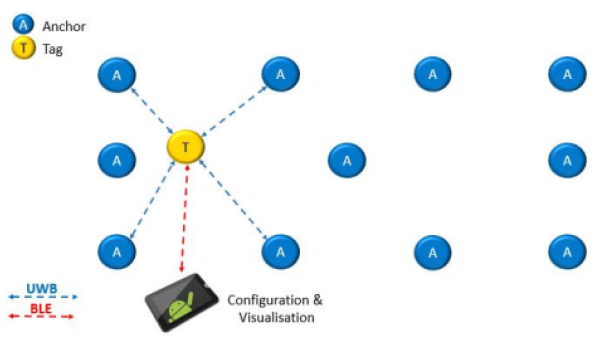
\includegraphics[width=1\textwidth]{image/decawave4ancres.png}}
            	\end{frame}
            	\caption{\label{fig:decawave4ancres}Représentation d'une configuration avec 1 tag et 11 ancres}
            \end{figure}
            
            \paragraph*{}
            Pour tester la méthode de Bancroft, j'ai utilisé la librairie fournie par l'Université du Texas à Austin (Space and Geophysics Laboraty (SGL)) qui se nomme GPSTk\cite{gpstk}. Cette librairie est Open Source et j'ai donc pu récupérer seulement la partie qui m'intéressait car la librairie entière permet des calculs avec l'orbite des planètes, satellites, etc. Elle est très complète mais était trop complète pour mon usage, j'ai donc récupéré seulement les fichiers servants à la méthode de Bancroft et je les ai inclus dans mon \rpi ~pour la compilation et l'exécution du code.
            
            Lors de ces essais, j'ai constaté que le positionnement des cartes et leur orientation jouaient un rôle assez important dans la précision et aussi dans la qualité du signal reçu par le drone et également des distances courtes entre chaque carte 'ancres' favorisaient de plus larges erreurs à cause du bruitage trop élevé.
        
        
        \paragraph{Méthode de Newton/Raphson}
            \paragraph*{}
            La méthode de Newton/Raphson est la méthode qui est probablement implémentée au sein des cartes Decawave par le constructeur. Il n'est pas possible de vérifier mais il est possible de faire des hypothèses notamment grâce au fait qu'il ne prenne que 4 cartes pour faire les calculs et jamais davantage.
            
            Cette méthode, itérative, est efficace pour trouver numériquement une approximation d'une fonction.
            
            \paragraph*{}
            Cette fonction appliquée dans l'environnement nous donne des résultats sans davantage de calculs avec une précision de l'ordre de 5 centimètres en moyenne si les distances des cartes sont plus élevés que ce que j'avais au départ pendant mes essais.
            
            Cette méthode étant simple à utiliser et très rapide car il est possible de l'avoir toutes les 100ms fait que je l'ai choisie par rapport à la méthode de Bancroft qui était très légère également mais avec des résultats très mauvais.
            
        
        \paragraph{Résultats}
            \paragraph*{}
            Pour présenter les différents résultats, je vais comparer les méthodes de Bancroft et celle de Newton/Raphson (Decawave). Les comparaisons se feront en terme de temps d'exécution pour voir si la méthode correspond aux exigences de temporalité demandée (période de 100ms), mais aussi avec la valeur de position calculée et l'écart par rapport à la réalité ainsi que la valeur moyenne et engin l'erreur moyenne calculée sur 1000 itérations.
            
            \paragraph*{}
            Comme il est possible de voir sur la figure \ref{fig:positionAncresTest}, le drone est positionné environ au milieu des ancres afin de tester. Le test se fait avec 7 ancres et un tag se trouvant sur le dessus du drone. Les valeurs de positions sous chaque ancre ou tag sont indiquées de cette façon : X, Y, Z. La distance entre l'ancre et le tag (trait en pointillé) est une distance mesurée avec un mètre et chaque position de drone est également mesurée au mètre par rapport à l'ancre de référence (ancre 0 en $\begin{bmatrix}0 & 0 & 0\end{bmatrix}$).
            
            \begin{figure}[H]
                \centering
            	\begin{frame}{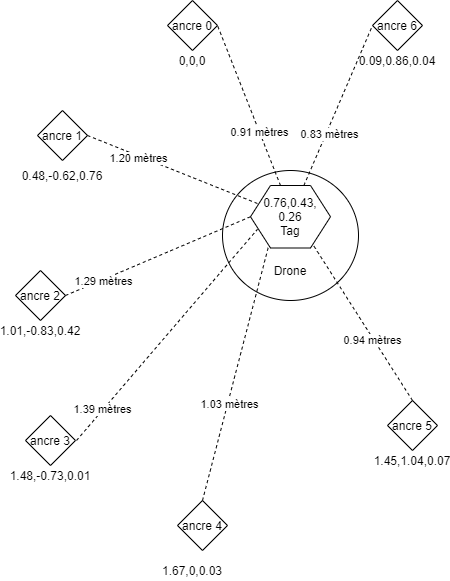
\includegraphics[width=0.8\textwidth]{image/positionnementAncres.png}}
            	\end{frame}
            	\caption{\label{fig:positionAncresTest}Schéma représentant le positionnement du drone et des ancres avec distance mesurée}
            \end{figure}
            
            \paragraph*{}
            Les résultats présentés sur le tableau \ref{table:resBancroft} montrent la comparaison de la valeur calculée par la méthode de Bancroft en utilisant 5 et 7 ancres actives par rapport à la réalité. Il est vrai comme indiqué précédemment que les cartes Decawaves ne prennent que 4 cartes en même temps, les résultats avec 5 et 7 sont possibles mais le tag ne prendra que 4 cartes, c'est juste qu'il aura le choix et donc choisira les plus proches ou d'autres selon la qualité du signal et donc on obtient des valeurs un peu plus précises.
            
            On voit donc que le temps d'exécution est très bon, d'un facteur entre 100 et 200 environ. Les résultats du vecteur sont par contre très approximatif. On peut constater qu'en X la valeur est très correct à 8 centimètres pour les 5 ancres et 5 centimètres pour les 7 ancres. Par contre, là où le problème se pose c'est au niveau du Y et Z qui là peut atteindre une erreur de 1 mètre 20 ! Cette erreur est impossible à maintenir pour une application.
            
            \begin{table}[H]
                \resizebox{\textwidth}{!}{
                    \begin{tabular}{| c | c | c |}
                        \hline
                        \textbf{Méthode} & \textbf{Temps d'exécution} & \textbf{Valeur du vecteur résultat} \\[0.15cm] \hline
                        Réalité & / & 0.76 0.43 0.26 \\[0.15cm]
                        \hline
                        Bancroft 7 ancres & entre 520 µs et 1200 µs & 0.71 0.80 0.78 \\[0.15cm]
                        \hline
                        Bancroft 5 ancres & entre 450 µs et 1200 µs & 0.68 1.37 1.46 \\[0.15cm]
                        \hline
                    \end{tabular}
                }
                \caption{\label{table:resBancroft}Résultats obtenus avec Bancroft}
            \end{table}
            
            \paragraph*{}
            Les résultats du tableau \ref{table:resAll} montrent la comparaison entre la réalité de la position du drone et la valeur calculée par Bancroft avec 4 ancres disponibles et Decawave avec 4 ancres également. Il est possible de voir que le temps d'exécution est très largement respecté pour les deux méthodes mais par contre la valeur du vecteur résultat est très différent selon les méthodes. La méthode de Bancroft prouve par ce tableau et ces résultats qu'elle n'est pas possible d'utilisation dans notre cas, peut-être car les distances sont trop petites. Pour avoir un ordre numérique de marge d'erreur, j'ai calculé la racine de l'erreur quadratique moyenne (RSME - Root Mean Square Error). La formule est : 
            \begin{equation} \label{maths:rsme}
                err=\sqrt{(posX-droneX)^{2}+(posY-droneY)^{2}+(posZ-droneZ)^{2}}
            \end{equation}
            
            Dans l'équation \ref{maths:rsme}, la valeur $\mathbf{posXYZ}$ correspond à la position calculée par la méthode (Bancroft ou Newton avec Decawave) que ce soit en X, Y ou Z; et $\mathbf{droneXYZ}$ correspond à la valeur réelle du drone en X, Y ou Z, cette valeur étant fixée manuellement dans le code pour les tests car le drone ne se déplaçait pas.
            
            \begin{table}[H]
                \resizebox{\textwidth}{!}{
                    \begin{tabular}{| c | c | c | c |}
                        \hline
                        \textbf{Méthode} & \textbf{Temps d'exécution} & \textbf{Valeur du vecteur résultat} & \textbf{RSME} \\[0.15cm] \hline
                        Réalité & / & 0.76 0.43 0.26 & / \\[0.15cm]
                        \hline
                        Bancroft & $\cong$ 840 µs & 0.98 -0.11 0.35 & 0.34 \\[0.15cm]
                        \hline
                        Decawave & $\cong$ 840 µs & 0.78 0.38 0.26 & 0.07 \\[0.15cm]
                        \hline
                    \end{tabular}
                }
                \caption{\label{table:resAll}Résultats obtenus avec Bancroft et Decawave}
            \end{table}
            
             \paragraph*{}
            Les résultats du tableau \ref{table:resMoyens} montrent les valeurs moyennes obtenues ainsi que l'erreur moyenne sur 1000 itérations de boucle. Ce calcul montre définitivement que Bancroft n'est pas utilisable, une erreur moyenne de 0.88 en Y est énorme et ne peut pas être utilisée. Alors que l'erreur pour Decawave ne dépasse pas les 0.08, ce qui est très bon comme résultat. Surtout que dans la suite du stage, la hauteur de déplacement du drone n'était pas forcément prise en compte car on peut également fixer le drone à une altitude de déplacement suffisamment haute pour éviter toute collision et le faire avancer en ligne droite sans devoir se repositionner en Z.
            
            \begin{table}[H]
                \resizebox{\textwidth}{!}{
                    \begin{tabular}{| c | c | c | c |}
                        \hline
                        \textbf{Méthode} & \textbf{Valeurs moyennes} & \textbf{Erreurs moyennes sur X, Y, Z} \\[0.15cm] \hline
                        Réalité & / & / \\[0.15cm]
                        \hline
                        Bancroft & \makecell{X = 0.98\\ Y = -0.11\\ Z = 0.35} & \makecell{X = 0.223\\ Y = 0.884 \\ Z = 0.418} \\
                        \hline
                        Decawave & \makecell{X = 0.77\\ Y = 0.38\\ Z = 0.26} & \makecell{X = 0.014\\ Y = 0.068\\ Z = 0.084}\\
                        \hline
                    \end{tabular}
                }
                \caption{\label{table:resMoyens}Résultats moyens obtenus avec Bancroft et Decawave}
            \end{table}
            
        
        \paragraph{Problèmes rencontrés}
            \paragraph*{}
            Dans cette partie, le plus gros soucis a été la connexion série en C++. Il n'existe pas de librairie qui le fasse facilement comme en Python avec pyserial. Il a donc fallu comprendre le fonctionnement et recréer les structures nécessaires grâce au site Web \textit{Linux Serial Ports Using C/C++}\cite{portSerieCpp}.
            
            
            \paragraph*{}
            Le second problème a été de trouver la meilleure solution de positionnement du drone. Comme j'ai pu montrer dans les paragraphes précédents, la méthode de Decawave au départ nous paraissait pas très précise alors qu'au final nous l'avons choisie car parmis les 2 méthodes testées c'était la meilleure en tout.
    
    \subsubsection{Drone : Déplacement dans la pièce}
        \paragraph*{}
        Le déplacement du drone a été choisie très simplement. La solution la plus directe c'est la ligne droite.
        
        Au départ, j'ai cherché une fonction dans le $SDK$ qui permettait de donner une trajectoire au drone de manière automatisée d'un point A à un point B. En partant du principe que le drone est orienté de la même façon tout le temps (voir figure \ref{fig:methodologie}) par exemple sur l'axe des X qui est fixé hypothétiquement sur l'axe Nord de la pièce.
        
        
        \begin{figure}[H]
            \centering
        	\begin{frame}{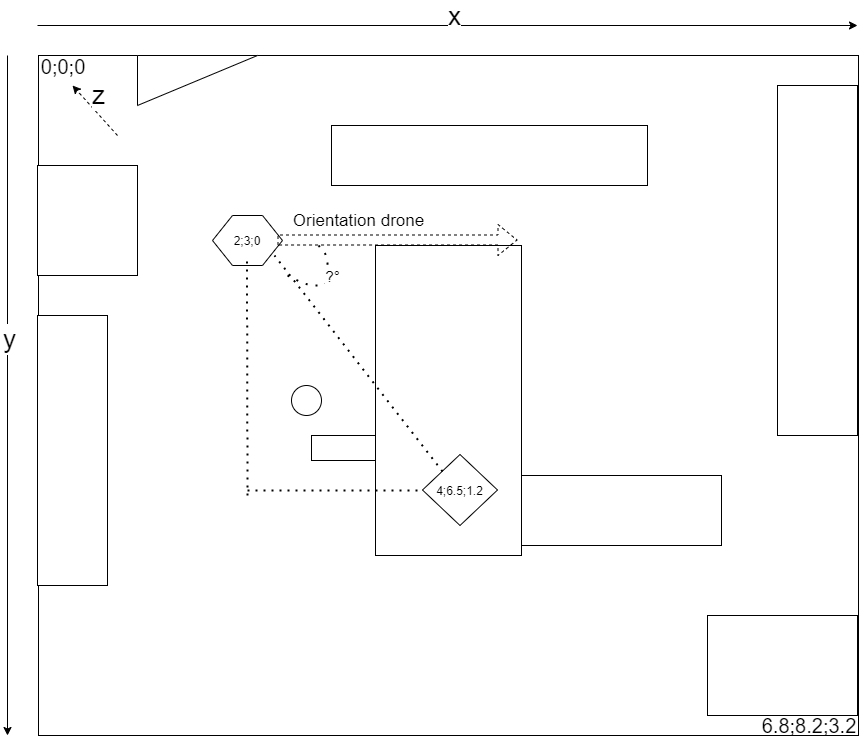
\includegraphics[width=1\textwidth]{image/methodologie.png}}
        	\end{frame}
        	\caption{\label{fig:methodologie}Schéma représentant l'orientation du drone par rapport au point d'arrivée}
        \end{figure}
        
        \paragraph*{}
        J'ai ainsi trouvé la fonction fournie (voir le bloc de code \ref{code:moveDrone}) par le constructeur qui permet un déplacement selon une distance en X, Y et Z avec possibilité de lui indiquer un angle de déplacement. Cette fonction correspondait parfaitement à mes attentes mais le soucis était de trouver l'angle de déplacement comme représenté sur la figure \ref{fig:methodologie}. On connait la position du drone, on connait la position du capteur mais l'angle de direction du drone est à déterminer sauf si on part de l'hypothèse que le drone est dans une direction fixe.
        
        Concernant l'axe Z, j'ai fait le choix, pendant le déplacement jusqu'au capteur, que le drone se positionne à une altitude donnée comme par exemple 2 mètres puis se tient sur cette altitude jusqu'au point et là réévalue l'altitude nécessaire pour la prise de la photo.
        
        \begin{lstlisting}[language=C++, caption=Fonction de déplacement du drone, label=code:moveDrone, aboveskip=1.7cm]
bool moveByPositionOffset(DJI::OSDK::Vehicle *vehicle,
    float xOffsetDesired,
    float yOffsetDesired,
    float zOffsetDesired,
    float yawDesired,
    float posThresholdInM = 0.5,
    float yawThresholdInDeg = 1.0);\end{lstlisting}
    
    
        \paragraph*{}
        Comme vu dans le paragraphe précédent, la fonction de déplacement demande un angle afin de s'orienter dans la direction. Le drone a parmis ses capteurs une boussole. Mais cette boussole doit être initialisée au départ du drone avec vue sur le ciel. Dans notre pièce, l'initialisation était impossible, ainsi à partir de ce moment il me fallait lancer le drone et l'initialiser dehors avec vue sur le ciel pour le calibrer.
        
        Dans la version du $SDK$ que j'utilise, il n'y a aucune fonction existante afin d'utiliser directement la boussole et la valeur renvoyée par le capteur. Par conséquence, je me suis orienter pour trouver une autre solution, un autre capteur sur le drone pour répondre à mes besoins. J'ai trouvé le magnétomètre et bien que la fonction soit notée seulement pour les drones \textit{M210V2} et \textit{M300}, la fonction fonctionne quand même sur mon drone. Malheureusement, les mesures étaient impossibles à deviner et la logique était compliquée à saisir sans avoir de documentation sur le fonctionnement précis de la fonction.
        
        \paragraph*{}
        %(voir compte rendu 13,14)
        Après davantage de recherches et d'explorations au sein de la documentation sommaire fournie ainsi que l'exploration directe du code à ma disposition dans les fichiers sources du $SDK$, j'ai trouvé une donnée qui correspond à une mesure de boussole.
        
        Cette mesure s'échelonnait de 0 à 0.9999 si on allait du Nord au Sud en passant par l'Est. Et si le drone allait du Nord au Sud en passant par l'Ouest, les mesures était de 0 à -0.9999. J'ai donc réalisé un étalonnage le plus précisément possible par rapport aux mesures que le drone nous donnait. Les résultats de ce relevé sont visibles sur la figure \ref{fig:roseVents} représentée par une rose des vents.
        
        
        \begin{figure}[H]
            \centering
        	\begin{frame}{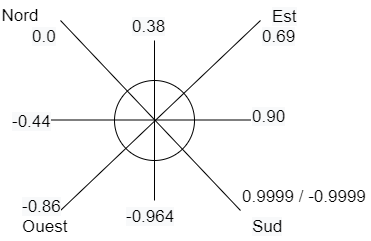
\includegraphics[width=0.8\textwidth]{image/roseVents.png}}
        	\end{frame}
        	\caption{\label{fig:roseVents}Schéma représentant les données du capteur selon l'angle du drone}
        \end{figure}
    
        \begin{figure}[H]
            \centering
        	\begin{frame}{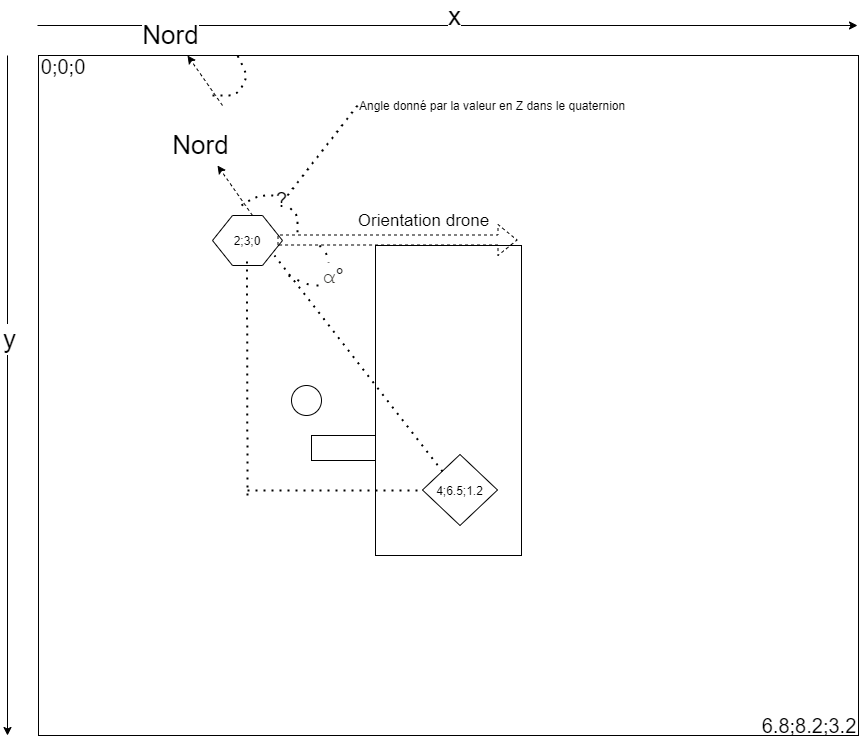
\includegraphics[width=0.8\textwidth]{image/angleNordDrone.png}}
        	\end{frame}
        	\caption{\label{fig:angleNordDrone}Schéma représentant l'angle à déterminer selon l'orientation du drone}
        \end{figure}
        
        
        \paragraph*{}
        Ainsi, pour finir le déplacement du drone d'un point A à un point B, je suis resté sur cette valeur qui n'est pas la plus précise mais qui est fiable malgré le contexte très défavorable de la pièce. Pour calibrer et étalonner la valeur reçue par rapport au drone, j'ai utilisé une fonction que j'ai récupéré d'Arduino qui se nomme \textit{map()} et qui prend une valeur en paramètre à réétalonner sur une autre échelle.
        
        \begin{lstlisting}[language=C++, caption=Exemple fonction map, label=code:mapArduino]
double map(double x, double in_min, double in_max, double out_min, double out_max){
	return (x - in_min) * (out_max - out_min) / (in_max - in_min) + out_min;
}
        
float angleReel = map(angle, 0.64, 0.90, 90, 135);\end{lstlisting}
        
        \paragraph*{}
        Comme on peut le voir sur le bloc de code \ref{code:mapArduino}, je pars d'une variable \textit{angle} qui prend une valeur entre 0.64 et 0.90 et je transforme cette valeur vers la nouvelle plage de valeur qui est entre 90 et 135 degrés.
        
        
    \subsubsection{Conclusion partielle}
        \paragraph*{}
        L'objectif de cette partie était de pouvoir accéder au drone depuis un ordinateur embarqué qui serait installé sur le drone. Cet ordinateur devait pouvoir gérer le déplacement, positionnement ainsi que la prise d'image ou l'analyse des images prises. L'ordinateur a donc été choisi avec ces contraintes. Un deuxième objectif était de pouvoir positionner le drone à l'intérieur de la pièce ainsi que de le faire se déplacer automatiquement d'un point de départ à un point d'arrivée avec le retour au point de départ ou un point qui serait déterminé comme base du drone.
        
        Pour réaliser tous ces objectifs, j'ai, grâce au \rpi, pu intégrer le $SDK$ du drone fourni par le constructeur DJI. Ce $SDK$ me permettait d'accéder à l'autopilote du drone et de gérer le déplacement du drone. Enfin, le positionnement s'est fait grâce à un moyen externe au drone. Les cartes Decawaves avec une communication $UWB$ m'ont permis de placer le drone de manière assez précise (erreur quadratique moyenne de 0.07) avec une déviation de seulement quelques centimètres.